\section{ĐỊNH NGHĨA, TÍNH CHẤT CỦA TÍCH PHÂN}
\subsection{LÝ THUYẾT CẦN NHỚ}
\subsubsection{Định nghĩa:}
\begin{enumerate}[\iconMT]
	\item \indam{Công thức tính:} \\
	\begin{minipage}[b]{8.5cm}
	Cho $f$ là một hàm số liên tục trên $[a;b]$. Giả sử $F(x)$ là một nguyên hàm của $f(x)$ trên $[a;b]$. Tích phân từ $a$ đến $b$ của $f(x)$, kí hiệu là $\displaystyle\int\limits_a^b f(x)\mathrm{\,d}x$ và được tính theo công thức sau:
	\boxmini{$\displaystyle\int\limits_a^b f(x)\mathrm{\,d}x=F(x)\bigg|_a^b=F(b)-F(a)$}
	\end{minipage}\hspace{1cm}
	\begin{minipage}[b]{7cm}
		\begin{khung4}{Chú ý}
			\begin{listEX}[1]
				\item [\ding{172}] $\displaystyle\int\limits_a^a{f(x)}\mathrm{\,d}x=0$.
				\item [\ding{173}] $-\displaystyle\int\limits_a^b{f(x)}\mathrm{\,d}x=\displaystyle\int\limits_b^a{f(x)}\mathrm{\,d}x$.
				\item [\ding{174}] $\displaystyle\int\limits_a^b{f(x)}\mathrm{\,d}x=\displaystyle\int\limits_a^b{f(t)}\mathrm{\,d}t$.
			\end{listEX}
		\end{khung4}
	\end{minipage}
\item \indam{Ý nghĩa hình học:}
\immini{Nếu hàm số $f(x)$ liên tục và không âm trên $[a;b]$ thì $\displaystyle\int\limits_a^b f(x)\mathrm{\,d}x$ là diện tích $S$ của \ind{hình thang cong} giới hạn bởi đồ thị $y=f(x)$, trục hoành, hai đường thẳng $x=a$ và $x=b$ (phần gạch sọc ở hình bên)
}{\hspace{1cm}
	\begin{tikzpicture}[smooth,samples=300,scale=0.7,>=stealth,font=\footnotesize]
		\draw[->] (-0.8,0)--(4.5,0) node[below]{$x$};
		\draw[->] (0,-0.5)--(0,3) node[right]{$y$};
		\draw (0,0) node[below left]{$O$};
		\draw[line width=0.7pt,domain=0.3:3.2] plot(\x,{0.3*(\x-1)^2+1})node[above right]{\scriptsize $y=f(x)$};
		\draw[fill=black] (1,0) circle(1pt) (3,0) circle(1pt);
		\draw[dashed] (1,0)node[below]{$a$}--(1,1) (3,0)node[below]{$b$}--(3,2.2);
		\fill[pattern=north west lines] (1,0)--plot[domain=1:3](\x,{0.3*(\x-1)^2+1})--(3,0)--cycle;
		\draw[->] (2.5,0.5)--(3.7,1) node[right]{$S$};
\end{tikzpicture}}
\begin{luuy} Một số lưu ý:
	\immini{
		\begin{itemize}
			\item [\ding{172}] Nếu $f(x) \le 0,\, \forall x \in [a;b]$ thì $\displaystyle\int\limits_a^b f(x)\mathrm{\,d}x=-S$
			\item [\ding{173}] Giả sử $f(x)$ liên tục trên $[a;c]$ và có đồ thị như hình bên. Gọi $S_1$, $S_2$ lần lượt là phần diện tích giới hạn bởi đồ thị $y=f(x)$ với trục hoành (hình vẽ). Khi đó
			\begin{center}
				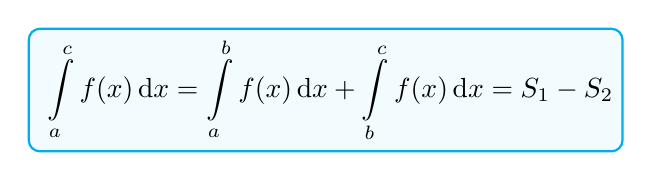
\begin{tikzpicture}[outline/.style={draw=#1,thick,fill=#1!5},
					outline/.default=cyan]
					\node [outline,rounded corners] at (0,0) {\fontfamily{qag} \selectfont\bfseries\color{black} $\displaystyle\int\limits_a^c f(x)\mathrm{\,d}x=\displaystyle\int\limits_a^b f(x)\mathrm{\,d}x+\displaystyle\int\limits_b^c f(x)\mathrm{\,d}x=S_1-S_2$};
				\end{tikzpicture}
			\end{center}
		\end{itemize}
	}{\vspace{1cm}
		\begin{tikzpicture}[smooth,samples=300,scale=0.8,>=stealth,font=\footnotesize]
			\draw[->] (-0.8,0)--(5,0) node[below]{$x$};
			\draw[->] (0,-1.5)--(0,2) node[right]{$y$};
			\draw (0,0) node[below left]{$O$};
			\draw[line width=0.7pt,domain=0.8:3.2] plot(\x,{2.2*(\x-1)*(\x-1.7)*(\x-3)})node[above right]{$y=f(x)$};
			\draw[fill=black] (1,0) circle(1pt) (1.7,0) circle(1pt) (3,0) circle(1pt);
			\fill[pattern = north west lines,smooth] (1,0)--plot[domain=1:1.7](\x,{2.2*(\x-1)*(\x-1.7)*(\x-3)})--(1.7,0);
			\fill[pattern = dots,smooth] (1.7,0)--plot[domain=1.7:3](\x,{2.2*(\x-1)*(\x-1.7)*(\x-3)})--(3,0);
			\node[below left] at (1,0) {$a$};
			\node[above right] at (1.7,0) {$b$};
			\node[below right] at (3,0) {$c$};
			\draw[->] (1.2,0.2)--(1.4,1.2) node[above]{$S_1$};
			\draw[->] (2.6,-0.5)--(3.4,-1.2) node[below right]{$S_2$};
	\end{tikzpicture}}
\end{luuy}
\end{enumerate}


